\section{Metadata feature library for quality traceability}\label{sec:extension}

\sideboxbegin{o}
This section presents the limitations imposed by the state of the art of KerML / SysMLv2 in terms of meta-annotation. It then presents the design that we have implemented to overcome it.
\sideboxend
We have previously mentioned the advantages that the use of feature libraries  (orthogonal) offers compared to more intrusive strategies (modifying the structure of the language).

However, the development of datatypes dedicated to traceability encounters a certain number of limitations due to the state of progress of the implementation of KerML / SysMLv2. In this section, we present the limitations encountered and then our design for quality traceability for KerML \textit{and} SysMLv2.

\subsection{Orthogonality - priority and limitations}\label{sec:orthogonalite}
 
\begin{figure}[ht]     
	\centering
	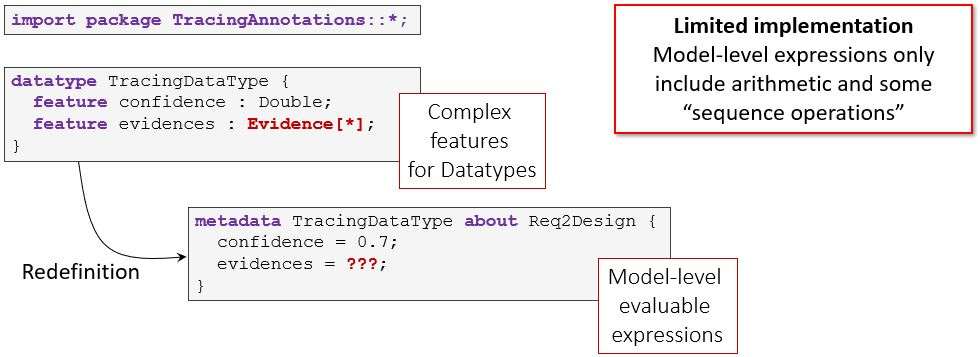
\includegraphics[width=.99\linewidth]{images/strategy4-metadatatype.jpg}
	\caption{Defining complex Metadata structures and evaluating expressions at model level: implementation limits. }
	\label{fig:strategy4}
\end{figure}


To use the words of Ed Seidewitz, one of the main promoters of the new version of SysML and one of the main people responsible for its delivery, the idea of using the AnnotatingFeatures to define \textit{a priori} external needs to the language specifications is "extremely relevant". However, the next revision will not contain any specific article on the matter. A number of decisions remain to be clarified on the subject.
In particular, the ability to define and reuse complex structures within feature datatypes is under consideration. For now, the definition of complex datatype is not guaranteed to work, as illustrated in \Fig{fig:strategy4}.

\begin{figure}[ht]     
	\centering
	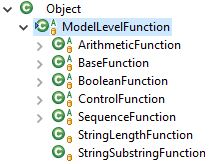
\includegraphics[width=.35\linewidth]{images/modellevelfunction-type-hierarchy.JPG}
	\caption{Types of functions available for evaluating expressions at the model level.}
	\label{fig:modellevelfunc}
\end{figure}

Until the delivery of the second revision (RFP2) scheduled for late August 2021, the SST remains busy with other priorities. Ed Seidewitz foresees the deployment of the features related to modelv level expression in October or November 2021. At the time of writing, annotating features are "only" templates in which some points of variability are allowed (the authorized functions are derived from ModelLevelFunction, see \Fig{fig:modellevelfunc}).

Consequently, the definition of complex structures within datatypes is limited as stated above. Only Ed Seidewitz is aware of the code related to the question and he himself struggles to remember the state of the module dedicated to the assignment of values to complex datatypes. As an example, the use of enumeration (\textit{enum}) in annotations does not allow their use for evaluation (see \Sect{sec:filter}). 
Finalizing this implementation will only be possible when a subset of the modeling language SysML will be defined. In view of the SST's plans to converge the different types of annotations towards AnnotatingFeatures using metadatatypes, these points will be addressed with high priority -- but only after the submission of the new revision.

\subsection{Iterative design: confidence and explainability of trace links}\label{sec:design}
\begin{figure}[ht]      
	\centering
	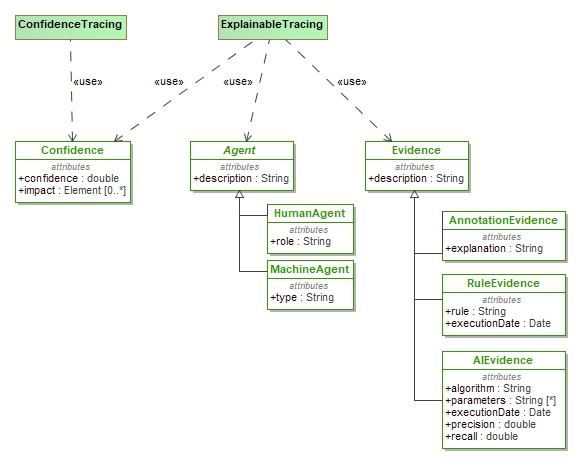
\includegraphics[width=.9\linewidth]{images/explainability-datatype.jpg}
	\caption{Metadatatypes for quality traceability including an assessment of confidence and monitoring of the identification processes used.}
	\label{fig:datatypes}
\end{figure}

To favor the use of specialized libraries (such as the SST encourages), we have designed SysML and KerML datatypes dedicated to tracing. 
\Fig{fig:datatypes} shows the design of these structures. At the top, we distinguish between a design allowing the assessment of confidence and a design allowing to go further by entering the supporting information for this assessment.
We distinguish between the two for the sake of iterativity of the development and implementation processes (as we have just seen, the mechanisms allowing the manipulation and evaluation of datatypes are not fully completed in KerML / SysMLv2).

The \texttt{ConfidenceTracing} datatype has been implemented to overcome this disappointment and initially allows the attribution of a real value of confidence to the annotated links. We add a description field (free String) and a field to reference to potentially impacted elements -- \textit{e.g.,} used in the calculation of the confidence value.
The \texttt{ExplainableTracing} datatype has the same attributes as ConfidenceTracing (description, confidence and impact) with in addition \textit{i)} the notion of Evidence to store information about the identification process used for tracing, and \textit{ii)} the possibility to inform which (type of) agent is responsible for identification.

\subsection{Consequence of the separation of KerML and SysML languages}\label{sec:lggsep}
SysML is based on KerML. However, if the language dedicated to systems reuses the concepts of the kernel language, these are not accessible from the former. Thus, the definition of a Datatype (and its associated Features) does not work in SysML but only in KerML. To allow the use of Trace\textit{a} in both languages, we have transformed the Datatypes and their features into \textit{attribute definitions and uses} (resp. "Attribute def" and "Attribute"). Indeed, an attribute definition is a particular type of structure dedicated to the construction of Datatypes for the design of systems (see \Fig{fig:dtnattributes}).


\begin{figure}[h]     
	\centering
	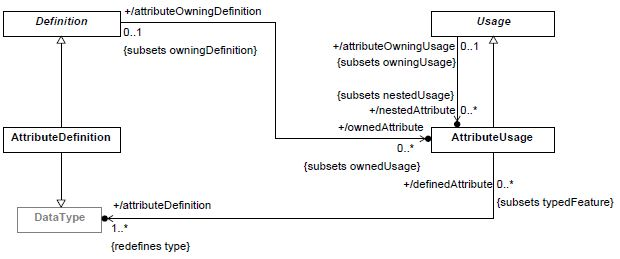
\includegraphics[width=.9\linewidth]{images/dtnattributes.JPG}
	\caption{The definition and use of attributes in SysML is a specialization of datatypes and their features in KerML.}
	\label{fig:dtnattributes}
\end{figure} 

\subsection{Usage example: filtering}\label{sec:filter}
This section presents an example: the filtering of links satisfying a confidence greater than a given threshold.
The first 30 lines of listing~\ref{lst:filter} (with graphical representation in \Fig{fig:vizfilter}), show the structure of the system and links being traced. Lines 33 to 39 show the code needed for filtering. This is a reuse of the existing machinery to support SysMLv2 metadata annotations. \Fig{fig:vizfilterres} shows the result of the query: the five links with a confidence greater than 0.5 are filtered.

% \pagebreak
\begin{lstlisting}[caption={Definition and filtering of tracing annotations to collect links satisfying a certain level of confidence.},
label=lst:filter,
style=mystylesysml,
linewidth=16cm,
xleftmargin=1.7cm,
morekeywords={part,filter}]
package Tracing_FilterExample {
	import TracingAnnotations::*;
	
	/* System under tracing. */
	part end1 {}
	part end2 {}
	part end3 {}
	part end4 {}
	part end5 {}
	part end6 {}
	part end7 {}
	part end8 {}
	
	/* Trace links, confidence valued. */
	connection testLink95 connect end1 to end2 
	  {@ConfidenceTracing { confidence = 0.95; }}
	connection testLink85 connect end1 to end3 
	  {@ConfidenceTracing { confidence = 0.85; }}
	connection testLink75 connect end1 to end4 
	  {@ConfidenceTracing { confidence = 0.75; }}
	connection testLink65 connect end5 to end6 
	  {@ConfidenceTracing { confidence = 0.65; }}
	connection testLink55 connect end6 to end7 
	  {@ConfidenceTracing { confidence = 0.55; }}
	connection testLink45 connect end7 to end8 
	  {@ConfidenceTracing { confidence = 0.45; }}
	connection testLink35 connect end8 to end7 
	  {@ConfidenceTracing { confidence = 0.35; }}
	connection testLink25 connect end8 to end6 
	  {@ConfidenceTracing { confidence = 0.25; }}
}

import TracingAnnotations::*;
/* Filter example - full notation. */
package ConfidenceLevel {
	/*Connections that satisfy a threshold confidence level (0.5).*/
    import Tracing_FilterExample::**;
    filter @ConfidenceTracing && ConfidenceTracing::confidence >= 0.5;
}
\end{lstlisting}


\begin{figure}[ht]     
	\centering
	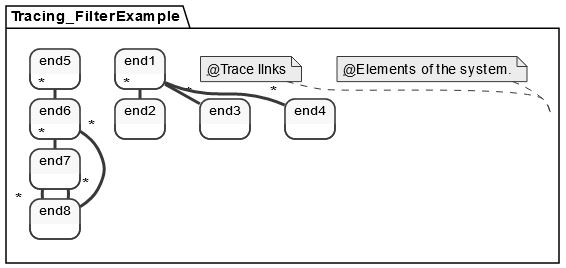
\includegraphics[width=.9\linewidth]{images/viz_filterexample.JPG}
	\caption{Example using the SysMLv2 filtering tool for trace annotations.}
	\label{fig:vizfilter}
\end{figure} 

\begin{figure}[ht]     
	\centering
	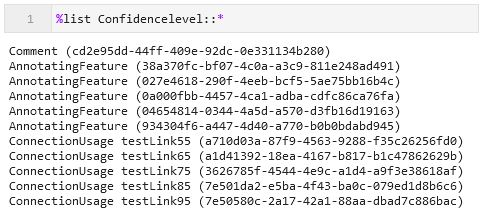
\includegraphics[width=.75\linewidth]{images/viz_filterexample_res.JPG}
	\caption{Filtering result: filtered annotations (\textit{i.e.,} satisfying a specific confidence).}
	\label{fig:vizfilterres}
\end{figure} 



The same process can (could) be used to "tag" links with specific types -- or any other pre-defined attribute. The implementation of the evaluation of expressions is unfortunately limited. As to this day, the use of strings of characters (\textit{String}) or of enumerations (\textit{enum}) in the definition of datatypes generates a compilation error. \Fig{fig:vizfiltererr} shows this limitation (the figure has been generated with JupyterLab, see \Sect{sec:artefacts}).

\begin{figure}[ht]     
	\centering
	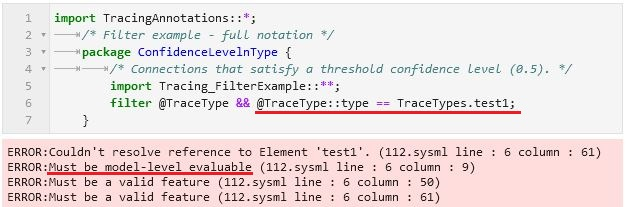
\includegraphics[width=.9\linewidth]{images/viz_filterexample_err.JPG}
	\caption{Filtering is not (yet) implemented for enumerations.}
	\label{fig:vizfiltererr}
\end{figure} 
